\documentclass[10pt,tikz,border=5pt]{standalone}
\usepackage[T1]{fontenc}
\usepackage{lmodern,amsmath,booktabs,array,tabularx,microtype,tikz}
\usetikzlibrary{patterns,patterns.meta,shapes.geometric,arrows.meta,calc,positioning}
\begin{document}
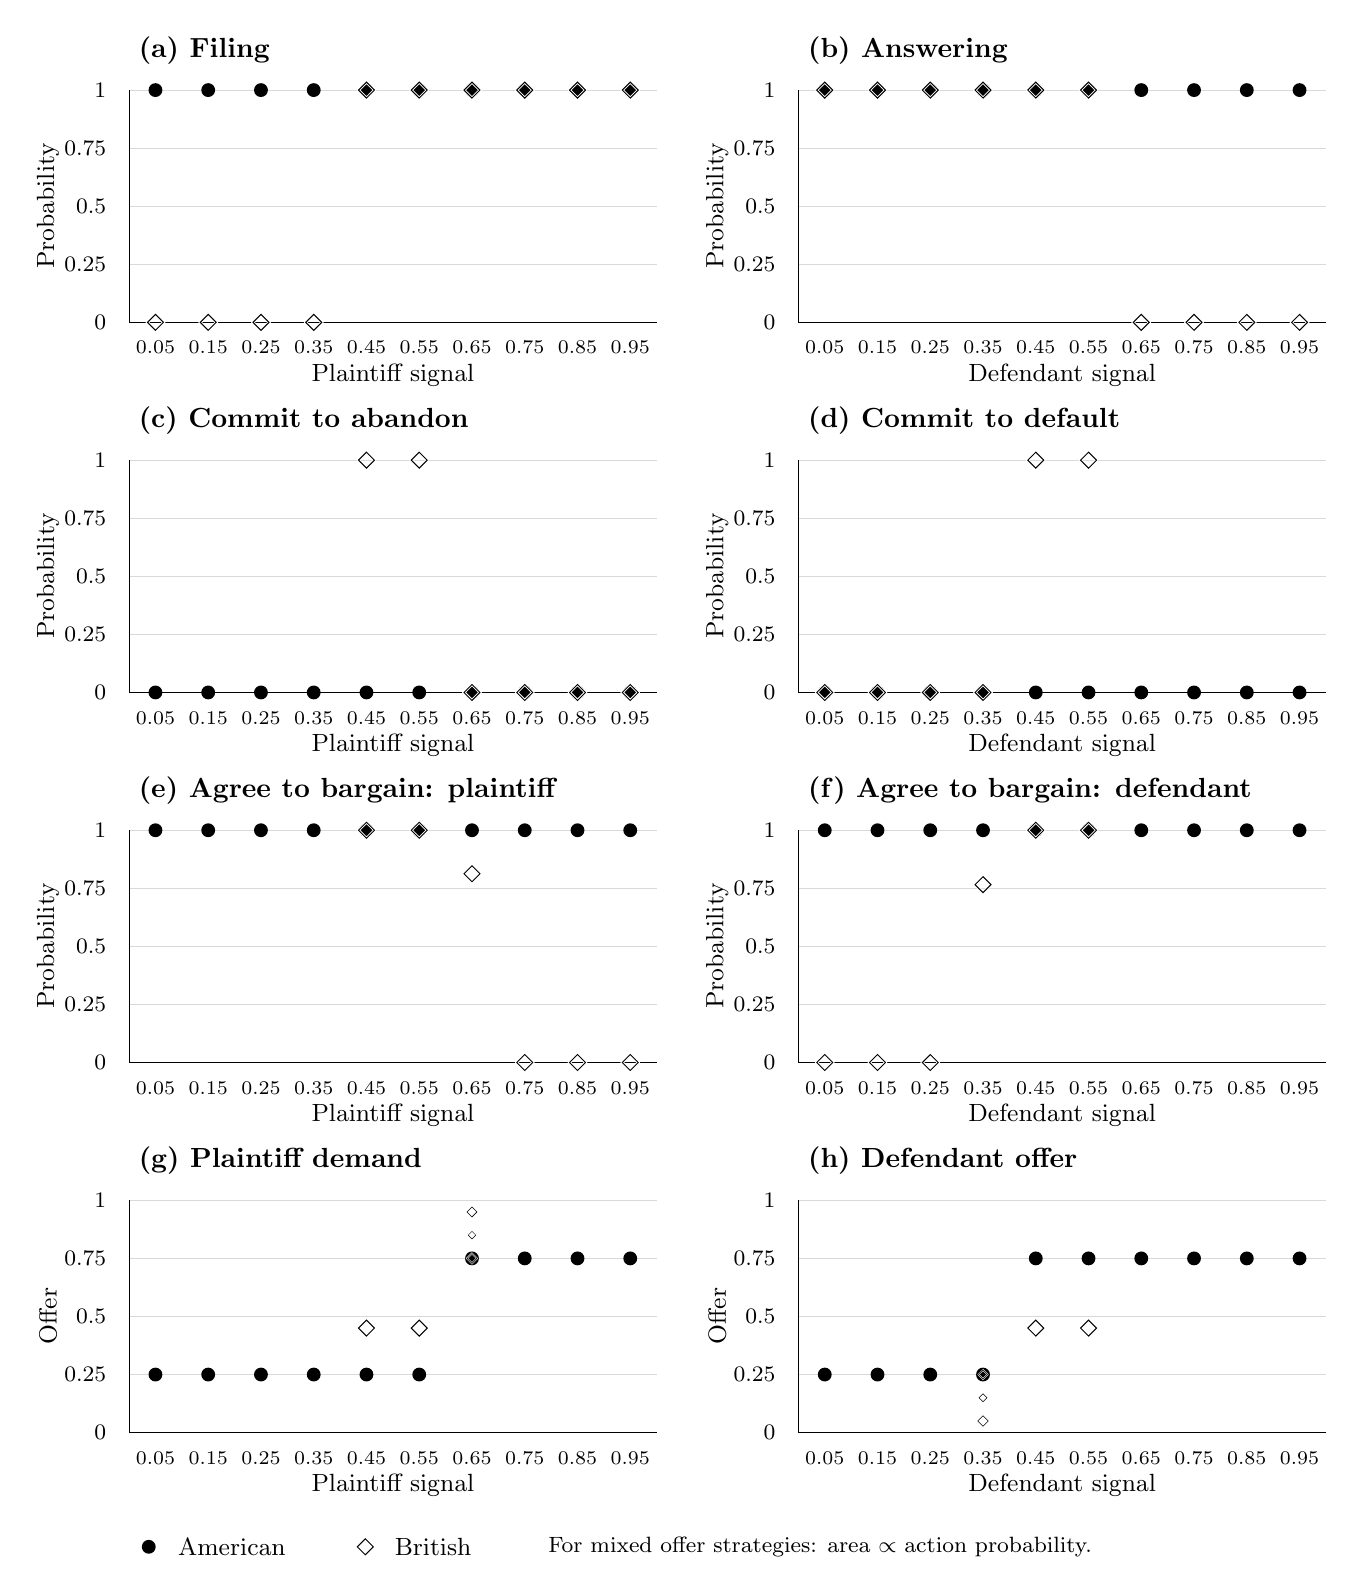
\begin{tikzpicture}[font=\small]
\node[anchor=west,font=\bfseries] at (1,18.550000000000001) {(a) Filing};
\begin{scope}[shift={(1,15.100000000000001)},x=6.7cm,y=2.95cm]
\draw[black!15] (0,0)--(1,0);
\node[anchor=east,font=\footnotesize] at (-.025,0) {0};
\draw[black!15] (0,0.25)--(1,0.25);
\node[anchor=east,font=\footnotesize] at (-.025,0.25) {0.25};
\draw[black!15] (0,0.5)--(1,0.5);
\node[anchor=east,font=\footnotesize] at (-.025,0.5) {0.5};
\draw[black!15] (0,0.75)--(1,0.75);
\node[anchor=east,font=\footnotesize] at (-.025,0.75) {0.75};
\draw[black!15] (0,1)--(1,1);
\node[anchor=east,font=\footnotesize] at (-.025,1) {1};
\draw (0,1)--(0,0)--(1,0);
\node[anchor=north,font=\scriptsize] at (0.05,-.04) {0.05};
\node[anchor=north,font=\scriptsize] at (0.15,-.04) {0.15};
\node[anchor=north,font=\scriptsize] at (0.25,-.04) {0.25};
\node[anchor=north,font=\scriptsize] at (0.35,-.04) {0.35};
\node[anchor=north,font=\scriptsize] at (0.45,-.04) {0.45};
\node[anchor=north,font=\scriptsize] at (0.55,-.04) {0.55};
\node[anchor=north,font=\scriptsize] at (0.65,-.04) {0.65};
\node[anchor=north,font=\scriptsize] at (0.75,-.04) {0.75};
\node[anchor=north,font=\scriptsize] at (0.85,-.04) {0.85};
\node[anchor=north,font=\scriptsize] at (0.95,-.04) {0.95};
\begin{scope}[shift={(0.05000000,1.00000000)}]\fill[black] (0pt,0pt) circle[radius=2.500000000pt];\end{scope}
\begin{scope}[shift={(0.15000000,1.00000000)}]\fill[black] (0pt,0pt) circle[radius=2.500000000pt];\end{scope}
\begin{scope}[shift={(0.25000000,1.00000000)}]\fill[black] (0pt,0pt) circle[radius=2.500000000pt];\end{scope}
\begin{scope}[shift={(0.35000000,1.00000000)}]\fill[black] (0pt,0pt) circle[radius=2.500000000pt];\end{scope}
\begin{scope}[shift={(0.45000000,1.00000000)}]\fill[black] (0pt,0pt) circle[radius=2.500000000pt];\end{scope}
\begin{scope}[shift={(0.55000000,1.00000000)}]\fill[black] (0pt,0pt) circle[radius=2.500000000pt];\end{scope}
\begin{scope}[shift={(0.65000000,1.00000000)}]\fill[black] (0pt,0pt) circle[radius=2.500000000pt];\end{scope}
\begin{scope}[shift={(0.75000000,1.00000000)}]\fill[black] (0pt,0pt) circle[radius=2.500000000pt];\end{scope}
\begin{scope}[shift={(0.85000000,1.00000000)}]\fill[black] (0pt,0pt) circle[radius=2.500000000pt];\end{scope}
\begin{scope}[shift={(0.95000000,1.00000000)}]\fill[black] (0pt,0pt) circle[radius=2.500000000pt];\end{scope}
\begin{scope}[shift={(0.05000000,0.00000000)}]\draw[draw=black,line width=0.350000000pt,line join=miter,miter limit=10,preaction={draw=white,line width=1.000000000pt,line join=miter}] (0pt,2.885797970pt)--(2.885797970pt,0pt)--(0pt,-2.885797970pt)--(-2.885797970pt,0pt)--cycle;\end{scope}
\begin{scope}[shift={(0.15000000,0.00000000)}]\draw[draw=black,line width=0.350000000pt,line join=miter,miter limit=10,preaction={draw=white,line width=1.000000000pt,line join=miter}] (0pt,2.885797970pt)--(2.885797970pt,0pt)--(0pt,-2.885797970pt)--(-2.885797970pt,0pt)--cycle;\end{scope}
\begin{scope}[shift={(0.25000000,0.00000000)}]\draw[draw=black,line width=0.350000000pt,line join=miter,miter limit=10,preaction={draw=white,line width=1.000000000pt,line join=miter}] (0pt,2.885797970pt)--(2.885797970pt,0pt)--(0pt,-2.885797970pt)--(-2.885797970pt,0pt)--cycle;\end{scope}
\begin{scope}[shift={(0.35000000,0.00000000)}]\draw[draw=black,line width=0.350000000pt,line join=miter,miter limit=10,preaction={draw=white,line width=1.000000000pt,line join=miter}] (0pt,2.885797970pt)--(2.885797970pt,0pt)--(0pt,-2.885797970pt)--(-2.885797970pt,0pt)--cycle;\end{scope}
\begin{scope}[shift={(0.45000000,1.00000000)}]\draw[draw=black,line width=0.350000000pt,line join=miter,miter limit=10,preaction={draw=white,line width=1.000000000pt,line join=miter}] (0pt,2.885797970pt)--(2.885797970pt,0pt)--(0pt,-2.885797970pt)--(-2.885797970pt,0pt)--cycle;\end{scope}
\begin{scope}[shift={(0.55000000,1.00000000)}]\draw[draw=black,line width=0.350000000pt,line join=miter,miter limit=10,preaction={draw=white,line width=1.000000000pt,line join=miter}] (0pt,2.885797970pt)--(2.885797970pt,0pt)--(0pt,-2.885797970pt)--(-2.885797970pt,0pt)--cycle;\end{scope}
\begin{scope}[shift={(0.65000000,1.00000000)}]\draw[draw=black,line width=0.350000000pt,line join=miter,miter limit=10,preaction={draw=white,line width=1.000000000pt,line join=miter}] (0pt,2.885797970pt)--(2.885797970pt,0pt)--(0pt,-2.885797970pt)--(-2.885797970pt,0pt)--cycle;\end{scope}
\begin{scope}[shift={(0.75000000,1.00000000)}]\draw[draw=black,line width=0.350000000pt,line join=miter,miter limit=10,preaction={draw=white,line width=1.000000000pt,line join=miter}] (0pt,2.885797970pt)--(2.885797970pt,0pt)--(0pt,-2.885797970pt)--(-2.885797970pt,0pt)--cycle;\end{scope}
\begin{scope}[shift={(0.85000000,1.00000000)}]\draw[draw=black,line width=0.350000000pt,line join=miter,miter limit=10,preaction={draw=white,line width=1.000000000pt,line join=miter}] (0pt,2.885797970pt)--(2.885797970pt,0pt)--(0pt,-2.885797970pt)--(-2.885797970pt,0pt)--cycle;\end{scope}
\begin{scope}[shift={(0.95000000,1.00000000)}]\draw[draw=black,line width=0.350000000pt,line join=miter,miter limit=10,preaction={draw=white,line width=1.000000000pt,line join=miter}] (0pt,2.885797970pt)--(2.885797970pt,0pt)--(0pt,-2.885797970pt)--(-2.885797970pt,0pt)--cycle;\end{scope}
\end{scope}
\node at (4.3499999999999996,14.430000000000001) {Plaintiff signal};
\node[rotate=90] at (-0.030000000000000027,16.580000000000002) {Probability};
\node[anchor=west,font=\bfseries] at (9.5,18.550000000000001) {(b) Answering};
\begin{scope}[shift={(9.5,15.100000000000001)},x=6.7cm,y=2.95cm]
\draw[black!15] (0,0)--(1,0);
\node[anchor=east,font=\footnotesize] at (-.025,0) {0};
\draw[black!15] (0,0.25)--(1,0.25);
\node[anchor=east,font=\footnotesize] at (-.025,0.25) {0.25};
\draw[black!15] (0,0.5)--(1,0.5);
\node[anchor=east,font=\footnotesize] at (-.025,0.5) {0.5};
\draw[black!15] (0,0.75)--(1,0.75);
\node[anchor=east,font=\footnotesize] at (-.025,0.75) {0.75};
\draw[black!15] (0,1)--(1,1);
\node[anchor=east,font=\footnotesize] at (-.025,1) {1};
\draw (0,1)--(0,0)--(1,0);
\node[anchor=north,font=\scriptsize] at (0.05,-.04) {0.05};
\node[anchor=north,font=\scriptsize] at (0.15,-.04) {0.15};
\node[anchor=north,font=\scriptsize] at (0.25,-.04) {0.25};
\node[anchor=north,font=\scriptsize] at (0.35,-.04) {0.35};
\node[anchor=north,font=\scriptsize] at (0.45,-.04) {0.45};
\node[anchor=north,font=\scriptsize] at (0.55,-.04) {0.55};
\node[anchor=north,font=\scriptsize] at (0.65,-.04) {0.65};
\node[anchor=north,font=\scriptsize] at (0.75,-.04) {0.75};
\node[anchor=north,font=\scriptsize] at (0.85,-.04) {0.85};
\node[anchor=north,font=\scriptsize] at (0.95,-.04) {0.95};
\begin{scope}[shift={(0.05000000,1.00000000)}]\fill[black] (0pt,0pt) circle[radius=2.500000000pt];\end{scope}
\begin{scope}[shift={(0.15000000,1.00000000)}]\fill[black] (0pt,0pt) circle[radius=2.500000000pt];\end{scope}
\begin{scope}[shift={(0.25000000,1.00000000)}]\fill[black] (0pt,0pt) circle[radius=2.500000000pt];\end{scope}
\begin{scope}[shift={(0.35000000,1.00000000)}]\fill[black] (0pt,0pt) circle[radius=2.500000000pt];\end{scope}
\begin{scope}[shift={(0.45000000,1.00000000)}]\fill[black] (0pt,0pt) circle[radius=2.500000000pt];\end{scope}
\begin{scope}[shift={(0.55000000,1.00000000)}]\fill[black] (0pt,0pt) circle[radius=2.500000000pt];\end{scope}
\begin{scope}[shift={(0.65000000,1.00000000)}]\fill[black] (0pt,0pt) circle[radius=2.500000000pt];\end{scope}
\begin{scope}[shift={(0.75000000,1.00000000)}]\fill[black] (0pt,0pt) circle[radius=2.500000000pt];\end{scope}
\begin{scope}[shift={(0.85000000,1.00000000)}]\fill[black] (0pt,0pt) circle[radius=2.500000000pt];\end{scope}
\begin{scope}[shift={(0.95000000,1.00000000)}]\fill[black] (0pt,0pt) circle[radius=2.500000000pt];\end{scope}
\begin{scope}[shift={(0.05000000,1.00000000)}]\draw[draw=black,line width=0.350000000pt,line join=miter,miter limit=10,preaction={draw=white,line width=1.000000000pt,line join=miter}] (0pt,2.885797970pt)--(2.885797970pt,0pt)--(0pt,-2.885797970pt)--(-2.885797970pt,0pt)--cycle;\end{scope}
\begin{scope}[shift={(0.15000000,1.00000000)}]\draw[draw=black,line width=0.350000000pt,line join=miter,miter limit=10,preaction={draw=white,line width=1.000000000pt,line join=miter}] (0pt,2.885797970pt)--(2.885797970pt,0pt)--(0pt,-2.885797970pt)--(-2.885797970pt,0pt)--cycle;\end{scope}
\begin{scope}[shift={(0.25000000,1.00000000)}]\draw[draw=black,line width=0.350000000pt,line join=miter,miter limit=10,preaction={draw=white,line width=1.000000000pt,line join=miter}] (0pt,2.885797970pt)--(2.885797970pt,0pt)--(0pt,-2.885797970pt)--(-2.885797970pt,0pt)--cycle;\end{scope}
\begin{scope}[shift={(0.35000000,1.00000000)}]\draw[draw=black,line width=0.350000000pt,line join=miter,miter limit=10,preaction={draw=white,line width=1.000000000pt,line join=miter}] (0pt,2.885797970pt)--(2.885797970pt,0pt)--(0pt,-2.885797970pt)--(-2.885797970pt,0pt)--cycle;\end{scope}
\begin{scope}[shift={(0.45000000,1.00000000)}]\draw[draw=black,line width=0.350000000pt,line join=miter,miter limit=10,preaction={draw=white,line width=1.000000000pt,line join=miter}] (0pt,2.885797970pt)--(2.885797970pt,0pt)--(0pt,-2.885797970pt)--(-2.885797970pt,0pt)--cycle;\end{scope}
\begin{scope}[shift={(0.55000000,1.00000000)}]\draw[draw=black,line width=0.350000000pt,line join=miter,miter limit=10,preaction={draw=white,line width=1.000000000pt,line join=miter}] (0pt,2.885797970pt)--(2.885797970pt,0pt)--(0pt,-2.885797970pt)--(-2.885797970pt,0pt)--cycle;\end{scope}
\begin{scope}[shift={(0.65000000,0.00000000)}]\draw[draw=black,line width=0.350000000pt,line join=miter,miter limit=10,preaction={draw=white,line width=1.000000000pt,line join=miter}] (0pt,2.885797970pt)--(2.885797970pt,0pt)--(0pt,-2.885797970pt)--(-2.885797970pt,0pt)--cycle;\end{scope}
\begin{scope}[shift={(0.75000000,0.00000000)}]\draw[draw=black,line width=0.350000000pt,line join=miter,miter limit=10,preaction={draw=white,line width=1.000000000pt,line join=miter}] (0pt,2.885797970pt)--(2.885797970pt,0pt)--(0pt,-2.885797970pt)--(-2.885797970pt,0pt)--cycle;\end{scope}
\begin{scope}[shift={(0.85000000,0.00000000)}]\draw[draw=black,line width=0.350000000pt,line join=miter,miter limit=10,preaction={draw=white,line width=1.000000000pt,line join=miter}] (0pt,2.885797970pt)--(2.885797970pt,0pt)--(0pt,-2.885797970pt)--(-2.885797970pt,0pt)--cycle;\end{scope}
\begin{scope}[shift={(0.95000000,0.00000000)}]\draw[draw=black,line width=0.350000000pt,line join=miter,miter limit=10,preaction={draw=white,line width=1.000000000pt,line join=miter}] (0pt,2.885797970pt)--(2.885797970pt,0pt)--(0pt,-2.885797970pt)--(-2.885797970pt,0pt)--cycle;\end{scope}
\end{scope}
\node at (12.85,14.430000000000001) {Defendant signal};
\node[rotate=90] at (8.4700000000000006,16.580000000000002) {Probability};
\node[anchor=west,font=\bfseries] at (1,13.850000000000001) {(c) Commit to abandon};
\begin{scope}[shift={(1,10.4)},x=6.7cm,y=2.95cm]
\draw[black!15] (0,0)--(1,0);
\node[anchor=east,font=\footnotesize] at (-.025,0) {0};
\draw[black!15] (0,0.25)--(1,0.25);
\node[anchor=east,font=\footnotesize] at (-.025,0.25) {0.25};
\draw[black!15] (0,0.5)--(1,0.5);
\node[anchor=east,font=\footnotesize] at (-.025,0.5) {0.5};
\draw[black!15] (0,0.75)--(1,0.75);
\node[anchor=east,font=\footnotesize] at (-.025,0.75) {0.75};
\draw[black!15] (0,1)--(1,1);
\node[anchor=east,font=\footnotesize] at (-.025,1) {1};
\draw (0,1)--(0,0)--(1,0);
\node[anchor=north,font=\scriptsize] at (0.05,-.04) {0.05};
\node[anchor=north,font=\scriptsize] at (0.15,-.04) {0.15};
\node[anchor=north,font=\scriptsize] at (0.25,-.04) {0.25};
\node[anchor=north,font=\scriptsize] at (0.35,-.04) {0.35};
\node[anchor=north,font=\scriptsize] at (0.45,-.04) {0.45};
\node[anchor=north,font=\scriptsize] at (0.55,-.04) {0.55};
\node[anchor=north,font=\scriptsize] at (0.65,-.04) {0.65};
\node[anchor=north,font=\scriptsize] at (0.75,-.04) {0.75};
\node[anchor=north,font=\scriptsize] at (0.85,-.04) {0.85};
\node[anchor=north,font=\scriptsize] at (0.95,-.04) {0.95};
\begin{scope}[shift={(0.05000000,0.00000000)}]\fill[black] (0pt,0pt) circle[radius=2.500000000pt];\end{scope}
\begin{scope}[shift={(0.15000000,0.00000000)}]\fill[black] (0pt,0pt) circle[radius=2.500000000pt];\end{scope}
\begin{scope}[shift={(0.25000000,0.00000000)}]\fill[black] (0pt,0pt) circle[radius=2.500000000pt];\end{scope}
\begin{scope}[shift={(0.35000000,0.00000000)}]\fill[black] (0pt,0pt) circle[radius=2.500000000pt];\end{scope}
\begin{scope}[shift={(0.45000000,0.00000000)}]\fill[black] (0pt,0pt) circle[radius=2.500000000pt];\end{scope}
\begin{scope}[shift={(0.55000000,0.00000000)}]\fill[black] (0pt,0pt) circle[radius=2.500000000pt];\end{scope}
\begin{scope}[shift={(0.65000000,0.00000000)}]\fill[black] (0pt,0pt) circle[radius=2.500000000pt];\end{scope}
\begin{scope}[shift={(0.75000000,0.00000000)}]\fill[black] (0pt,0pt) circle[radius=2.500000000pt];\end{scope}
\begin{scope}[shift={(0.85000000,0.00000000)}]\fill[black] (0pt,0pt) circle[radius=2.500000000pt];\end{scope}
\begin{scope}[shift={(0.95000000,0.00000000)}]\fill[black] (0pt,0pt) circle[radius=2.500000000pt];\end{scope}
\begin{scope}[shift={(0.45000000,1.00000000)}]\draw[draw=black,line width=0.350000000pt,line join=miter,miter limit=10,preaction={draw=white,line width=1.000000000pt,line join=miter}] (0pt,2.885797970pt)--(2.885797970pt,0pt)--(0pt,-2.885797970pt)--(-2.885797970pt,0pt)--cycle;\end{scope}
\begin{scope}[shift={(0.55000000,1.00000000)}]\draw[draw=black,line width=0.350000000pt,line join=miter,miter limit=10,preaction={draw=white,line width=1.000000000pt,line join=miter}] (0pt,2.885797970pt)--(2.885797970pt,0pt)--(0pt,-2.885797970pt)--(-2.885797970pt,0pt)--cycle;\end{scope}
\begin{scope}[shift={(0.65000000,0.00000000)}]\draw[draw=black,line width=0.350000000pt,line join=miter,miter limit=10,preaction={draw=white,line width=1.000000000pt,line join=miter}] (0pt,2.885797970pt)--(2.885797970pt,0pt)--(0pt,-2.885797970pt)--(-2.885797970pt,0pt)--cycle;\end{scope}
\begin{scope}[shift={(0.75000000,0.00000000)}]\draw[draw=black,line width=0.350000000pt,line join=miter,miter limit=10,preaction={draw=white,line width=1.000000000pt,line join=miter}] (0pt,2.885797970pt)--(2.885797970pt,0pt)--(0pt,-2.885797970pt)--(-2.885797970pt,0pt)--cycle;\end{scope}
\begin{scope}[shift={(0.85000000,0.00000000)}]\draw[draw=black,line width=0.350000000pt,line join=miter,miter limit=10,preaction={draw=white,line width=1.000000000pt,line join=miter}] (0pt,2.885797970pt)--(2.885797970pt,0pt)--(0pt,-2.885797970pt)--(-2.885797970pt,0pt)--cycle;\end{scope}
\begin{scope}[shift={(0.95000000,0.00000000)}]\draw[draw=black,line width=0.350000000pt,line join=miter,miter limit=10,preaction={draw=white,line width=1.000000000pt,line join=miter}] (0pt,2.885797970pt)--(2.885797970pt,0pt)--(0pt,-2.885797970pt)--(-2.885797970pt,0pt)--cycle;\end{scope}
\end{scope}
\node at (4.3499999999999996,9.7300000000000004) {Plaintiff signal};
\node[rotate=90] at (-0.030000000000000027,11.880000000000001) {Probability};
\node[anchor=west,font=\bfseries] at (9.5,13.850000000000001) {(d) Commit to default};
\begin{scope}[shift={(9.5,10.4)},x=6.7cm,y=2.95cm]
\draw[black!15] (0,0)--(1,0);
\node[anchor=east,font=\footnotesize] at (-.025,0) {0};
\draw[black!15] (0,0.25)--(1,0.25);
\node[anchor=east,font=\footnotesize] at (-.025,0.25) {0.25};
\draw[black!15] (0,0.5)--(1,0.5);
\node[anchor=east,font=\footnotesize] at (-.025,0.5) {0.5};
\draw[black!15] (0,0.75)--(1,0.75);
\node[anchor=east,font=\footnotesize] at (-.025,0.75) {0.75};
\draw[black!15] (0,1)--(1,1);
\node[anchor=east,font=\footnotesize] at (-.025,1) {1};
\draw (0,1)--(0,0)--(1,0);
\node[anchor=north,font=\scriptsize] at (0.05,-.04) {0.05};
\node[anchor=north,font=\scriptsize] at (0.15,-.04) {0.15};
\node[anchor=north,font=\scriptsize] at (0.25,-.04) {0.25};
\node[anchor=north,font=\scriptsize] at (0.35,-.04) {0.35};
\node[anchor=north,font=\scriptsize] at (0.45,-.04) {0.45};
\node[anchor=north,font=\scriptsize] at (0.55,-.04) {0.55};
\node[anchor=north,font=\scriptsize] at (0.65,-.04) {0.65};
\node[anchor=north,font=\scriptsize] at (0.75,-.04) {0.75};
\node[anchor=north,font=\scriptsize] at (0.85,-.04) {0.85};
\node[anchor=north,font=\scriptsize] at (0.95,-.04) {0.95};
\begin{scope}[shift={(0.05000000,0.00000000)}]\fill[black] (0pt,0pt) circle[radius=2.500000000pt];\end{scope}
\begin{scope}[shift={(0.15000000,0.00000000)}]\fill[black] (0pt,0pt) circle[radius=2.500000000pt];\end{scope}
\begin{scope}[shift={(0.25000000,0.00000000)}]\fill[black] (0pt,0pt) circle[radius=2.500000000pt];\end{scope}
\begin{scope}[shift={(0.35000000,0.00000000)}]\fill[black] (0pt,0pt) circle[radius=2.500000000pt];\end{scope}
\begin{scope}[shift={(0.45000000,0.00000000)}]\fill[black] (0pt,0pt) circle[radius=2.500000000pt];\end{scope}
\begin{scope}[shift={(0.55000000,0.00000000)}]\fill[black] (0pt,0pt) circle[radius=2.500000000pt];\end{scope}
\begin{scope}[shift={(0.65000000,0.00000000)}]\fill[black] (0pt,0pt) circle[radius=2.500000000pt];\end{scope}
\begin{scope}[shift={(0.75000000,0.00000000)}]\fill[black] (0pt,0pt) circle[radius=2.500000000pt];\end{scope}
\begin{scope}[shift={(0.85000000,0.00000000)}]\fill[black] (0pt,0pt) circle[radius=2.500000000pt];\end{scope}
\begin{scope}[shift={(0.95000000,0.00000000)}]\fill[black] (0pt,0pt) circle[radius=2.500000000pt];\end{scope}
\begin{scope}[shift={(0.05000000,0.00000000)}]\draw[draw=black,line width=0.350000000pt,line join=miter,miter limit=10,preaction={draw=white,line width=1.000000000pt,line join=miter}] (0pt,2.885797970pt)--(2.885797970pt,0pt)--(0pt,-2.885797970pt)--(-2.885797970pt,0pt)--cycle;\end{scope}
\begin{scope}[shift={(0.15000000,0.00000000)}]\draw[draw=black,line width=0.350000000pt,line join=miter,miter limit=10,preaction={draw=white,line width=1.000000000pt,line join=miter}] (0pt,2.885797970pt)--(2.885797970pt,0pt)--(0pt,-2.885797970pt)--(-2.885797970pt,0pt)--cycle;\end{scope}
\begin{scope}[shift={(0.25000000,0.00000000)}]\draw[draw=black,line width=0.350000000pt,line join=miter,miter limit=10,preaction={draw=white,line width=1.000000000pt,line join=miter}] (0pt,2.885797970pt)--(2.885797970pt,0pt)--(0pt,-2.885797970pt)--(-2.885797970pt,0pt)--cycle;\end{scope}
\begin{scope}[shift={(0.35000000,0.00000000)}]\draw[draw=black,line width=0.350000000pt,line join=miter,miter limit=10,preaction={draw=white,line width=1.000000000pt,line join=miter}] (0pt,2.885797970pt)--(2.885797970pt,0pt)--(0pt,-2.885797970pt)--(-2.885797970pt,0pt)--cycle;\end{scope}
\begin{scope}[shift={(0.45000000,1.00000000)}]\draw[draw=black,line width=0.350000000pt,line join=miter,miter limit=10,preaction={draw=white,line width=1.000000000pt,line join=miter}] (0pt,2.885797970pt)--(2.885797970pt,0pt)--(0pt,-2.885797970pt)--(-2.885797970pt,0pt)--cycle;\end{scope}
\begin{scope}[shift={(0.55000000,1.00000000)}]\draw[draw=black,line width=0.350000000pt,line join=miter,miter limit=10,preaction={draw=white,line width=1.000000000pt,line join=miter}] (0pt,2.885797970pt)--(2.885797970pt,0pt)--(0pt,-2.885797970pt)--(-2.885797970pt,0pt)--cycle;\end{scope}
\end{scope}
\node at (12.85,9.7300000000000004) {Defendant signal};
\node[rotate=90] at (8.4700000000000006,11.880000000000001) {Probability};
\node[anchor=west,font=\bfseries] at (1,9.1500000000000004) {(e) Agree to bargain: plaintiff};
\begin{scope}[shift={(1,5.7000000000000002)},x=6.7cm,y=2.95cm]
\draw[black!15] (0,0)--(1,0);
\node[anchor=east,font=\footnotesize] at (-.025,0) {0};
\draw[black!15] (0,0.25)--(1,0.25);
\node[anchor=east,font=\footnotesize] at (-.025,0.25) {0.25};
\draw[black!15] (0,0.5)--(1,0.5);
\node[anchor=east,font=\footnotesize] at (-.025,0.5) {0.5};
\draw[black!15] (0,0.75)--(1,0.75);
\node[anchor=east,font=\footnotesize] at (-.025,0.75) {0.75};
\draw[black!15] (0,1)--(1,1);
\node[anchor=east,font=\footnotesize] at (-.025,1) {1};
\draw (0,1)--(0,0)--(1,0);
\node[anchor=north,font=\scriptsize] at (0.05,-.04) {0.05};
\node[anchor=north,font=\scriptsize] at (0.15,-.04) {0.15};
\node[anchor=north,font=\scriptsize] at (0.25,-.04) {0.25};
\node[anchor=north,font=\scriptsize] at (0.35,-.04) {0.35};
\node[anchor=north,font=\scriptsize] at (0.45,-.04) {0.45};
\node[anchor=north,font=\scriptsize] at (0.55,-.04) {0.55};
\node[anchor=north,font=\scriptsize] at (0.65,-.04) {0.65};
\node[anchor=north,font=\scriptsize] at (0.75,-.04) {0.75};
\node[anchor=north,font=\scriptsize] at (0.85,-.04) {0.85};
\node[anchor=north,font=\scriptsize] at (0.95,-.04) {0.95};
\begin{scope}[shift={(0.05000000,1.00000000)}]\fill[black] (0pt,0pt) circle[radius=2.500000000pt];\end{scope}
\begin{scope}[shift={(0.15000000,1.00000000)}]\fill[black] (0pt,0pt) circle[radius=2.500000000pt];\end{scope}
\begin{scope}[shift={(0.25000000,1.00000000)}]\fill[black] (0pt,0pt) circle[radius=2.500000000pt];\end{scope}
\begin{scope}[shift={(0.35000000,1.00000000)}]\fill[black] (0pt,0pt) circle[radius=2.500000000pt];\end{scope}
\begin{scope}[shift={(0.45000000,1.00000000)}]\fill[black] (0pt,0pt) circle[radius=2.500000000pt];\end{scope}
\begin{scope}[shift={(0.55000000,1.00000000)}]\fill[black] (0pt,0pt) circle[radius=2.500000000pt];\end{scope}
\begin{scope}[shift={(0.65000000,1.00000000)}]\fill[black] (0pt,0pt) circle[radius=2.500000000pt];\end{scope}
\begin{scope}[shift={(0.75000000,1.00000000)}]\fill[black] (0pt,0pt) circle[radius=2.500000000pt];\end{scope}
\begin{scope}[shift={(0.85000000,1.00000000)}]\fill[black] (0pt,0pt) circle[radius=2.500000000pt];\end{scope}
\begin{scope}[shift={(0.95000000,1.00000000)}]\fill[black] (0pt,0pt) circle[radius=2.500000000pt];\end{scope}
\begin{scope}[shift={(0.45000000,1.00000000)}]\draw[draw=black,line width=0.350000000pt,line join=miter,miter limit=10,preaction={draw=white,line width=1.000000000pt,line join=miter}] (0pt,2.885797970pt)--(2.885797970pt,0pt)--(0pt,-2.885797970pt)--(-2.885797970pt,0pt)--cycle;\end{scope}
\begin{scope}[shift={(0.55000000,1.00000000)}]\draw[draw=black,line width=0.350000000pt,line join=miter,miter limit=10,preaction={draw=white,line width=1.000000000pt,line join=miter}] (0pt,2.885797970pt)--(2.885797970pt,0pt)--(0pt,-2.885797970pt)--(-2.885797970pt,0pt)--cycle;\end{scope}
\begin{scope}[shift={(0.65000000,0.81281900)}]\draw[draw=black,line width=0.350000000pt,line join=miter,miter limit=10,preaction={draw=white,line width=1.000000000pt,line join=miter}] (0pt,2.885797970pt)--(2.885797970pt,0pt)--(0pt,-2.885797970pt)--(-2.885797970pt,0pt)--cycle;\end{scope}
\begin{scope}[shift={(0.75000000,0.00000000)}]\draw[draw=black,line width=0.350000000pt,line join=miter,miter limit=10,preaction={draw=white,line width=1.000000000pt,line join=miter}] (0pt,2.885797970pt)--(2.885797970pt,0pt)--(0pt,-2.885797970pt)--(-2.885797970pt,0pt)--cycle;\end{scope}
\begin{scope}[shift={(0.85000000,0.00000000)}]\draw[draw=black,line width=0.350000000pt,line join=miter,miter limit=10,preaction={draw=white,line width=1.000000000pt,line join=miter}] (0pt,2.885797970pt)--(2.885797970pt,0pt)--(0pt,-2.885797970pt)--(-2.885797970pt,0pt)--cycle;\end{scope}
\begin{scope}[shift={(0.95000000,0.00000000)}]\draw[draw=black,line width=0.350000000pt,line join=miter,miter limit=10,preaction={draw=white,line width=1.000000000pt,line join=miter}] (0pt,2.885797970pt)--(2.885797970pt,0pt)--(0pt,-2.885797970pt)--(-2.885797970pt,0pt)--cycle;\end{scope}
\end{scope}
\node at (4.3499999999999996,5.0300000000000002) {Plaintiff signal};
\node[rotate=90] at (-0.030000000000000027,7.1799999999999997) {Probability};
\node[anchor=west,font=\bfseries] at (9.5,9.1500000000000004) {(f) Agree to bargain: defendant};
\begin{scope}[shift={(9.5,5.7000000000000002)},x=6.7cm,y=2.95cm]
\draw[black!15] (0,0)--(1,0);
\node[anchor=east,font=\footnotesize] at (-.025,0) {0};
\draw[black!15] (0,0.25)--(1,0.25);
\node[anchor=east,font=\footnotesize] at (-.025,0.25) {0.25};
\draw[black!15] (0,0.5)--(1,0.5);
\node[anchor=east,font=\footnotesize] at (-.025,0.5) {0.5};
\draw[black!15] (0,0.75)--(1,0.75);
\node[anchor=east,font=\footnotesize] at (-.025,0.75) {0.75};
\draw[black!15] (0,1)--(1,1);
\node[anchor=east,font=\footnotesize] at (-.025,1) {1};
\draw (0,1)--(0,0)--(1,0);
\node[anchor=north,font=\scriptsize] at (0.05,-.04) {0.05};
\node[anchor=north,font=\scriptsize] at (0.15,-.04) {0.15};
\node[anchor=north,font=\scriptsize] at (0.25,-.04) {0.25};
\node[anchor=north,font=\scriptsize] at (0.35,-.04) {0.35};
\node[anchor=north,font=\scriptsize] at (0.45,-.04) {0.45};
\node[anchor=north,font=\scriptsize] at (0.55,-.04) {0.55};
\node[anchor=north,font=\scriptsize] at (0.65,-.04) {0.65};
\node[anchor=north,font=\scriptsize] at (0.75,-.04) {0.75};
\node[anchor=north,font=\scriptsize] at (0.85,-.04) {0.85};
\node[anchor=north,font=\scriptsize] at (0.95,-.04) {0.95};
\begin{scope}[shift={(0.05000000,1.00000000)}]\fill[black] (0pt,0pt) circle[radius=2.500000000pt];\end{scope}
\begin{scope}[shift={(0.15000000,1.00000000)}]\fill[black] (0pt,0pt) circle[radius=2.500000000pt];\end{scope}
\begin{scope}[shift={(0.25000000,1.00000000)}]\fill[black] (0pt,0pt) circle[radius=2.500000000pt];\end{scope}
\begin{scope}[shift={(0.35000000,1.00000000)}]\fill[black] (0pt,0pt) circle[radius=2.500000000pt];\end{scope}
\begin{scope}[shift={(0.45000000,1.00000000)}]\fill[black] (0pt,0pt) circle[radius=2.500000000pt];\end{scope}
\begin{scope}[shift={(0.55000000,1.00000000)}]\fill[black] (0pt,0pt) circle[radius=2.500000000pt];\end{scope}
\begin{scope}[shift={(0.65000000,1.00000000)}]\fill[black] (0pt,0pt) circle[radius=2.500000000pt];\end{scope}
\begin{scope}[shift={(0.75000000,1.00000000)}]\fill[black] (0pt,0pt) circle[radius=2.500000000pt];\end{scope}
\begin{scope}[shift={(0.85000000,1.00000000)}]\fill[black] (0pt,0pt) circle[radius=2.500000000pt];\end{scope}
\begin{scope}[shift={(0.95000000,1.00000000)}]\fill[black] (0pt,0pt) circle[radius=2.500000000pt];\end{scope}
\begin{scope}[shift={(0.05000000,0.00000000)}]\draw[draw=black,line width=0.350000000pt,line join=miter,miter limit=10,preaction={draw=white,line width=1.000000000pt,line join=miter}] (0pt,2.885797970pt)--(2.885797970pt,0pt)--(0pt,-2.885797970pt)--(-2.885797970pt,0pt)--cycle;\end{scope}
\begin{scope}[shift={(0.15000000,0.00000000)}]\draw[draw=black,line width=0.350000000pt,line join=miter,miter limit=10,preaction={draw=white,line width=1.000000000pt,line join=miter}] (0pt,2.885797970pt)--(2.885797970pt,0pt)--(0pt,-2.885797970pt)--(-2.885797970pt,0pt)--cycle;\end{scope}
\begin{scope}[shift={(0.25000000,0.00000000)}]\draw[draw=black,line width=0.350000000pt,line join=miter,miter limit=10,preaction={draw=white,line width=1.000000000pt,line join=miter}] (0pt,2.885797970pt)--(2.885797970pt,0pt)--(0pt,-2.885797970pt)--(-2.885797970pt,0pt)--cycle;\end{scope}
\begin{scope}[shift={(0.35000000,0.76582995)}]\draw[draw=black,line width=0.350000000pt,line join=miter,miter limit=10,preaction={draw=white,line width=1.000000000pt,line join=miter}] (0pt,2.885797970pt)--(2.885797970pt,0pt)--(0pt,-2.885797970pt)--(-2.885797970pt,0pt)--cycle;\end{scope}
\begin{scope}[shift={(0.45000000,1.00000000)}]\draw[draw=black,line width=0.350000000pt,line join=miter,miter limit=10,preaction={draw=white,line width=1.000000000pt,line join=miter}] (0pt,2.885797970pt)--(2.885797970pt,0pt)--(0pt,-2.885797970pt)--(-2.885797970pt,0pt)--cycle;\end{scope}
\begin{scope}[shift={(0.55000000,1.00000000)}]\draw[draw=black,line width=0.350000000pt,line join=miter,miter limit=10,preaction={draw=white,line width=1.000000000pt,line join=miter}] (0pt,2.885797970pt)--(2.885797970pt,0pt)--(0pt,-2.885797970pt)--(-2.885797970pt,0pt)--cycle;\end{scope}
\end{scope}
\node at (12.85,5.0300000000000002) {Defendant signal};
\node[rotate=90] at (8.4700000000000006,7.1799999999999997) {Probability};
\node[anchor=west,font=\bfseries] at (1,4.4500000000000002) {(g) Plaintiff demand};
\begin{scope}[shift={(1,1)},x=6.7cm,y=2.95cm]
\draw[black!15] (0,0)--(1,0);
\node[anchor=east,font=\footnotesize] at (-.025,0) {0};
\draw[black!15] (0,0.25)--(1,0.25);
\node[anchor=east,font=\footnotesize] at (-.025,0.25) {0.25};
\draw[black!15] (0,0.5)--(1,0.5);
\node[anchor=east,font=\footnotesize] at (-.025,0.5) {0.5};
\draw[black!15] (0,0.75)--(1,0.75);
\node[anchor=east,font=\footnotesize] at (-.025,0.75) {0.75};
\draw[black!15] (0,1)--(1,1);
\node[anchor=east,font=\footnotesize] at (-.025,1) {1};
\draw (0,1)--(0,0)--(1,0);
\node[anchor=north,font=\scriptsize] at (0.05,-.04) {0.05};
\node[anchor=north,font=\scriptsize] at (0.15,-.04) {0.15};
\node[anchor=north,font=\scriptsize] at (0.25,-.04) {0.25};
\node[anchor=north,font=\scriptsize] at (0.35,-.04) {0.35};
\node[anchor=north,font=\scriptsize] at (0.45,-.04) {0.45};
\node[anchor=north,font=\scriptsize] at (0.55,-.04) {0.55};
\node[anchor=north,font=\scriptsize] at (0.65,-.04) {0.65};
\node[anchor=north,font=\scriptsize] at (0.75,-.04) {0.75};
\node[anchor=north,font=\scriptsize] at (0.85,-.04) {0.85};
\node[anchor=north,font=\scriptsize] at (0.95,-.04) {0.95};
\begin{scope}[shift={(0.05000000,0.25000000)}]\fill[black] (0pt,0pt) circle[radius=2.500000000pt];\end{scope}
\begin{scope}[shift={(0.15000000,0.25000000)}]\fill[black] (0pt,0pt) circle[radius=2.500000000pt];\end{scope}
\begin{scope}[shift={(0.25000000,0.25000000)}]\fill[black] (0pt,0pt) circle[radius=2.500000000pt];\end{scope}
\begin{scope}[shift={(0.35000000,0.25000000)}]\fill[black] (0pt,0pt) circle[radius=2.500000000pt];\end{scope}
\begin{scope}[shift={(0.45000000,0.25000000)}]\fill[black] (0pt,0pt) circle[radius=2.500000000pt];\end{scope}
\begin{scope}[shift={(0.55000000,0.25000000)}]\fill[black] (0pt,0pt) circle[radius=2.500000000pt];\end{scope}
\begin{scope}[shift={(0.65000000,0.75000000)}]\fill[black] (0pt,0pt) circle[radius=2.500000000pt];\end{scope}
\begin{scope}[shift={(0.75000000,0.75000000)}]\fill[black] (0pt,0pt) circle[radius=2.500000000pt];\end{scope}
\begin{scope}[shift={(0.85000000,0.75000000)}]\fill[black] (0pt,0pt) circle[radius=2.500000000pt];\end{scope}
\begin{scope}[shift={(0.95000000,0.75000000)}]\fill[black] (0pt,0pt) circle[radius=2.500000000pt];\end{scope}
\begin{scope}[shift={(0.45000000,0.45000000)}]\draw[draw=black,line width=0.350000000pt,line join=miter,miter limit=10,preaction={draw=white,line width=1.000000000pt,line join=miter}] (0pt,2.885797970pt)--(2.885797970pt,0pt)--(0pt,-2.885797970pt)--(-2.885797970pt,0pt)--cycle;\end{scope}
\begin{scope}[shift={(0.55000000,0.45000000)}]\draw[draw=black,line width=0.350000000pt,line join=miter,miter limit=10,preaction={draw=white,line width=1.000000000pt,line join=miter}] (0pt,2.885797970pt)--(2.885797970pt,0pt)--(0pt,-2.885797970pt)--(-2.885797970pt,0pt)--cycle;\end{scope}
\begin{scope}[shift={(0.65000000,0.75000000)}]\draw[draw=black,line width=0.216532159pt,line join=miter,miter limit=10,preaction={draw=white,line width=0.618663312pt,line join=miter}] (0pt,1.785337329pt)--(1.785337329pt,0pt)--(0pt,-1.785337329pt)--(-1.785337329pt,0pt)--cycle;\end{scope}
\begin{scope}[shift={(0.65000000,0.85000000)}]\draw[draw=black,line width=0.167728653pt,line join=miter,miter limit=10,preaction={draw=white,line width=0.479224722pt,line join=miter}] (0pt,1.382945731pt)--(1.382945731pt,0pt)--(0pt,-1.382945731pt)--(-1.382945731pt,0pt)--cycle;\end{scope}
\begin{scope}[shift={(0.65000000,0.95000000)}]\draw[draw=black,line width=0.217901177pt,line join=miter,miter limit=10,preaction={draw=white,line width=0.622574792pt,line join=miter}] (0pt,1.796625072pt)--(1.796625072pt,0pt)--(0pt,-1.796625072pt)--(-1.796625072pt,0pt)--cycle;\end{scope}
\end{scope}
\node at (4.3499999999999996,0.32999999999999996) {Plaintiff signal};
\node[rotate=90] at (-0.030000000000000027,2.48) {Offer};
\node[anchor=west,font=\bfseries] at (9.5,4.4500000000000002) {(h) Defendant offer};
\begin{scope}[shift={(9.5,1)},x=6.7cm,y=2.95cm]
\draw[black!15] (0,0)--(1,0);
\node[anchor=east,font=\footnotesize] at (-.025,0) {0};
\draw[black!15] (0,0.25)--(1,0.25);
\node[anchor=east,font=\footnotesize] at (-.025,0.25) {0.25};
\draw[black!15] (0,0.5)--(1,0.5);
\node[anchor=east,font=\footnotesize] at (-.025,0.5) {0.5};
\draw[black!15] (0,0.75)--(1,0.75);
\node[anchor=east,font=\footnotesize] at (-.025,0.75) {0.75};
\draw[black!15] (0,1)--(1,1);
\node[anchor=east,font=\footnotesize] at (-.025,1) {1};
\draw (0,1)--(0,0)--(1,0);
\node[anchor=north,font=\scriptsize] at (0.05,-.04) {0.05};
\node[anchor=north,font=\scriptsize] at (0.15,-.04) {0.15};
\node[anchor=north,font=\scriptsize] at (0.25,-.04) {0.25};
\node[anchor=north,font=\scriptsize] at (0.35,-.04) {0.35};
\node[anchor=north,font=\scriptsize] at (0.45,-.04) {0.45};
\node[anchor=north,font=\scriptsize] at (0.55,-.04) {0.55};
\node[anchor=north,font=\scriptsize] at (0.65,-.04) {0.65};
\node[anchor=north,font=\scriptsize] at (0.75,-.04) {0.75};
\node[anchor=north,font=\scriptsize] at (0.85,-.04) {0.85};
\node[anchor=north,font=\scriptsize] at (0.95,-.04) {0.95};
\begin{scope}[shift={(0.05000000,0.25000000)}]\fill[black] (0pt,0pt) circle[radius=2.500000000pt];\end{scope}
\begin{scope}[shift={(0.15000000,0.25000000)}]\fill[black] (0pt,0pt) circle[radius=2.500000000pt];\end{scope}
\begin{scope}[shift={(0.25000000,0.25000000)}]\fill[black] (0pt,0pt) circle[radius=2.500000000pt];\end{scope}
\begin{scope}[shift={(0.35000000,0.25000000)}]\fill[black] (0pt,0pt) circle[radius=2.500000000pt];\end{scope}
\begin{scope}[shift={(0.45000000,0.75000000)}]\fill[black] (0pt,0pt) circle[radius=2.500000000pt];\end{scope}
\begin{scope}[shift={(0.55000000,0.75000000)}]\fill[black] (0pt,0pt) circle[radius=2.500000000pt];\end{scope}
\begin{scope}[shift={(0.65000000,0.75000000)}]\fill[black] (0pt,0pt) circle[radius=2.500000000pt];\end{scope}
\begin{scope}[shift={(0.75000000,0.75000000)}]\fill[black] (0pt,0pt) circle[radius=2.500000000pt];\end{scope}
\begin{scope}[shift={(0.85000000,0.75000000)}]\fill[black] (0pt,0pt) circle[radius=2.500000000pt];\end{scope}
\begin{scope}[shift={(0.95000000,0.75000000)}]\fill[black] (0pt,0pt) circle[radius=2.500000000pt];\end{scope}
\begin{scope}[shift={(0.35000000,0.05000000)}]\draw[draw=black,line width=0.229698157pt,line join=miter,miter limit=10,preaction={draw=white,line width=0.656280448pt,line join=miter}] (0pt,1.893892786pt)--(1.893892786pt,0pt)--(0pt,-1.893892786pt)--(-1.893892786pt,0pt)--cycle;\end{scope}
\begin{scope}[shift={(0.35000000,0.15000000)}]\draw[draw=black,line width=0.176843441pt,line join=miter,miter limit=10,preaction={draw=white,line width=0.505266975pt,line join=miter}] (0pt,1.458098410pt)--(1.458098410pt,0pt)--(0pt,-1.458098410pt)--(-1.458098410pt,0pt)--cycle;\end{scope}
\begin{scope}[shift={(0.35000000,0.25000000)}]\draw[draw=black,line width=0.196125353pt,line join=miter,miter limit=10,preaction={draw=white,line width=0.560358151pt,line join=miter}] (0pt,1.617080414pt)--(1.617080414pt,0pt)--(0pt,-1.617080414pt)--(-1.617080414pt,0pt)--cycle;\end{scope}
\begin{scope}[shift={(0.45000000,0.45000000)}]\draw[draw=black,line width=0.350000000pt,line join=miter,miter limit=10,preaction={draw=white,line width=1.000000000pt,line join=miter}] (0pt,2.885797970pt)--(2.885797970pt,0pt)--(0pt,-2.885797970pt)--(-2.885797970pt,0pt)--cycle;\end{scope}
\begin{scope}[shift={(0.55000000,0.45000000)}]\draw[draw=black,line width=0.350000000pt,line join=miter,miter limit=10,preaction={draw=white,line width=1.000000000pt,line join=miter}] (0pt,2.885797970pt)--(2.885797970pt,0pt)--(0pt,-2.885797970pt)--(-2.885797970pt,0pt)--cycle;\end{scope}
\end{scope}
\node at (12.85,0.32999999999999996) {Defendant signal};
\node[rotate=90] at (8.4700000000000006,2.48) {Offer};
\begin{scope}[shift={(1.25000000,-0.45000000)}]\fill[black] (0pt,0pt) circle[radius=2.500000000pt];\end{scope}
\node[anchor=west] at (1.5,-.45) {American};
\begin{scope}[shift={(4.00000000,-0.45000000)}]\draw[draw=black,line width=0.350000000pt,line join=miter,miter limit=10,preaction={draw=white,line width=1.000000000pt,line join=miter}] (0pt,2.885797970pt)--(2.885797970pt,0pt)--(0pt,-2.885797970pt)--(-2.885797970pt,0pt)--cycle;\end{scope}
\node[anchor=west] at (4.25,-.45) {British};
\node[anchor=west,font=\footnotesize,align=left] at (6.2,-.45) {For mixed offer strategies: area $\propto$ action probability.};
\end{tikzpicture}
\end{document}